\documentclass[aps,pra,reprint,superscriptaddress,amsmath,amssymb,longbibliography]{revtex4-2}

\usepackage{graphicx}
\usepackage{xcolor}
\usepackage{booktabs}
\usepackage{bm}
\usepackage[colorlinks=true,linkcolor=blue!60!black,citecolor=blue!60!black,urlcolor=blue!60!black]{hyperref}

% generated by make_paper.py
\newcommand{\EHFabs}{-2.861\,679\,995\,612\,238\,878\,775\,543\,740\,022\,563\,429\,412\,879\,776\,752\,447\,053\,906\,864\ldots}
\newcommand{\EHFsplit}{\mathord{-}2.861\,679\,995\,612\,238\,878\,775\\ &\hphantom{-2.}543\,740\,022\,563\,429\,412\,879\\ &\hphantom{-2.}776\,752\,447\,053\,906\,864\,697}
\newcommand{\Ecorrsplit}{\mathord{-}0.042\,044\,381\,421\,880\,719\,535\\ &\hphantom{-0.}615\,505\,171\,841\,017\,284\,045\\ &\hphantom{-0.}534\,364\,843\,285\,135\,48}
\newcommand{\Nsf}{503}
\newcommand{\sfcert}{503.2}
\newcommand{\gapcert}{1.70\times10^{-503}}
\newcommand{\certvsa}{-2.6\times10^{-509}}
\newcommand{\Eamb}{1.70\times10^{-503}}
\newcommand{\Eapred}{1.7\times10^{-503}}
\newcommand{\Ecpred}{3\times10^{-519}}
\newcommand{\sfab}{503.2}
\newcommand{\virratio}{1168}
\newcommand{\twokR}{1170}
\newcommand{\virgap}{2.0\times10^{-500}}
\newcommand{\rstar}{-1.099\pm0.577\,i}
\newcommand{\rstarabs}{1.241}
\newcommand{\rstarerr}{7\times10^{-4}}
\newcommand{\kappaHe}{1.354958}
\newcommand{\sigmaHe}{0.7380}
\newcommand{\epsHe}{-0.9179555628563395101}
\newcommand{\tauHe}{1.0815}
\newcommand{\zetaopt}{4.98}
\newcommand{\digitsopt}{73}
\newcommand{\geoHatano}{70}
\newcommand{\singHatano}{74}
\newcommand{\Nfive}{2\,800}
\newcommand{\zetafive}{13}
\newcommand{\Ecorr}{-0.042\,044\,381\,421\,880\,719\,535\,615\,505\,171\,841\,017\,284\,045\,534\,364\,843\,285\,135\,48}
\newcommand{\Ncorr}{58}
\newcommand{\epsH}{-0.0462224456276869354}
\newcommand{\kappaH}{0.3040}
\newcommand{\EAH}{0.0120702656}
\newcommand{\plateau}{45}
\newcommand{\orderA}{164}
\newcommand{\Rone}{108.77}
\newcommand{\stepsRunA}{41}
\newcommand{\secRunA}{11}
\newcommand{\certRunA}{16}
\newcommand{\sfRunA}{124}
\newcommand{\stepsA}{51}
\newcommand{\stepsB}{30}
\newcommand{\minA}{7.4}
\newcommand{\minB}{8.2}
\newcommand{\BeNsf}{501}
\newcommand{\BeD}{500}
\newcommand{\BeEabs}{-14.573\,023\,168\,316\,399\,582\,411\,447\,359\,870\,014\,453\,877\,721\,357\ldots}
\newcommand{\BeEsplit}{\mathord{-}14.573\,023\,168\,316\,399\,582\\ &\hphantom{-14.}411\,447\,359\,870\,014\,453\\ &\hphantom{-14.}877\,721\,357\,774\,005\,413}
\newcommand{\BeSfcert}{501.3}
\newcommand{\BeGap}{7.08\times10^{-501}}
\newcommand{\BeEpsOne}{-4.73266989745572620396}
\newcommand{\BeEpsTwo}{-0.30926955157344281760}
\newcommand{\BeKappaOne}{3.077}
\newcommand{\BeKappaTwo}{0.786}
\newcommand{\BeSij}{4.9\times10^{-315}}
\newcommand{\BeRone}{190.1}
\newcommand{\BeRtwo}{743.7}
\newcommand{\BeTime}{4.0~hours}
\newcommand{\BeCertTime}{13~minutes}
\newcommand{\BeWallPred}{7.03\times10^{-501}}
\newcommand{\BeWallFrom}{100}
\newcommand{\BeRef}{500}
\newcommand{\MaxOrder}{873}
\newcommand{\PropRho}{500}
\newcommand{\PropRtwo}{500}
\newcommand{\PropR}{497}
\newcommand{\PropVR}{500}
\newcommand{\PropRtwelve}{474}
\newcommand{\PredParts}{5}
\newcommand{\TailBest}{261}
\newcommand{\Rfit}{222}
\newcommand{\Aasym}{1.39080116285695292083}
\newcommand{\UniPct}{0.04}
\newcommand{\BeOrbMin}{315}
\newcommand{\BeOrbMax}{321}
\newcommand{\BeDensMin}{478}
\newcommand{\BeDensMax}{498}
\newcommand{\BeRho}{498}

\newcommand{\eh}{E_\mathrm{h}}
\newcommand{\EHF}{E_\mathrm{HF}}

\begin{document}

\title{FROST: certified Hartree--Fock limits of helium and beryllium to hundreds of significant figures}

\author{Adam L. Baskerville}
% TODO: affiliation and e-mail
\noaffiliation

\begin{abstract}
We report rigorous upper bounds on the closed-shell Hartree--Fock (HF) energies of helium and beryllium whose first 503 and \BeNsf\ significant figures are correct,
\begin{align*}
\EHF(\mathrm{He}) &= \EHFabs\ \eh ,\\
\EHF(\mathrm{Be}) &= \BeEabs\ \eh ,
\end{align*}
against previous records of 66 and 43. The method, which we call FROST (Fock radial orbital shooting with Taylor series), uses no basis set. When every occupied orbital is an $s$ orbital, the HF equations reduce to coupled radial differential equations for the orbitals and for one potential per pair of orbitals. We integrate them with Taylor series of order up to \MaxOrder\ in arbitrary-precision arithmetic, sizing every step from the local radius of convergence. The orbital energies and normalisations are fixed by nested secant shooting to a hard wall, which is the only truncation and whose error decays as $e^{-2\kappa R}$. For beryllium each orbital has its own wall, and the canonical equations are solved without enforcing exact orthogonality, which costs energy far below the wall error. The orbitals are piecewise polynomials with dyadic rational coefficients. An independent program therefore evaluates the exact determinant energy in integer arithmetic, and by the variational principle the result is an upper bound free of rounding error. The orbitals are as accurate as the energies. Their nuclear cusp is exact, and for helium the density at the nucleus and $\langle r^k\rangle$ are obtained to about 500 significant figures (previously 32 to 65), with a pointwise error given in closed form by Whittaker functions. On a laptop, the 503-digit helium calculation takes 7.4 minutes and beryllium to \BeD\ digits \BeTime. The same code gives the HF energies of H$^-$ through Ne$^{8+}$ to 100 significant figures in about 15 seconds each. We locate the nearest singularities of the helium HF orbital in the complex plane at $r_*=\rstar$. This explains why single-exponent Laguerre-type bases converge sub-geometrically and predicts the optimised exponent of the previous record to within 3\%. Combined with our FLAKE energy, the correlation energy of helium follows to \Ncorr\ significant figures.
\end{abstract}

\maketitle

%=====================================================================================
\section{Introduction}
%=====================================================================================

The Hartree--Fock (HF) approximation is the oldest working model of a many-electron atom, yet is still widely used throughout quantum chemistry. In 1928, just two years after Schr\"odinger's equation, Hartree proposed that each electron moves in the field of the nucleus and the averaged charge of the other electrons, with that field iterated until the orbitals it produces regenerate it~\cite{Hartree1928}. Slater showed that this self-consistent field follows from the variational principle~\cite{Slater1928} and Fock~\cite{Fock1930} and Slater~\cite{Slater1930} then took the trial function to be an antisymmetrised product of orbitals, a determinant~\cite{Slater1929}, which satisfies the Pauli principle and adds an exchange term to Hartree's equations. For atoms these are radial differential equations, and they were first solved by integrating them numerically, step by step, on desk calculators. The calculation of Hartree and his father on beryllium~\cite{Hartree1935} was one of the first to include exchange, and the methods of that period are collected in Hartree's book~\cite{Hartree1957}.

A major advancement later came from Roothaan~\cite{Roothaan1951} and Hall~\cite{Hall1951} who turned the HF equations into a matrix eigenvalue problem by expanding the orbitals in a fixed basis. With Gaussian functions, whose many-centre integrals have closed forms~\cite{Boys1950}, this made HF calculations on molecules practical once electronic computers became available, and the basis-set expansion has been the standard route ever since. The HF determinant became the reference state of correlated electronic-structure theory; perturbation theory~\cite{Moller1934}, configuration interaction and coupled cluster~\cite{Cizek1966} all expand about it, and Kohn--Sham density functional theory~\cite{KohnSham1965} keeps its single-determinant form, with hybrid functionals using its exchange energy directly~\cite{Becke1993}. L\"owdin defined the correlation energy as what the HF limit misses, $E_\mathrm{corr}=E-\EHF$~\cite{Lowdin1959}. A correlation energy is therefore only as accurate as the HF limit it is measured from.

For atoms the radial equations can still be solved without explicitly using a basis. Numerical HF programs, notably that of Froese Fischer~\cite{FroeseFischer1977}, together with analytical Slater-type expansions~\cite{Roothaan1960,Clementi1974}, became the references against which basis sets are judged. The closed-shell $1s^2$ ground state of helium is the simplest of these problems and is a key focus of the work presented here. It has a single radial orbital, has been solved by almost every method devised for atomic structure, and its HF limit is the standard test of numerical HF methods and basis sets.

\begin{table*}[t]
\caption{Published Hartree--Fock energies of the helium ground state (hartree). Values before this work are as compiled in Table~4 of Ref.~\cite{Hatano2025}, where each is truncated to its number of correct significant figures (s.f.). Our row shows the first 71 of the 503 correct figures; Appendix~\ref{app:digits} gives all of them.}
\label{tab:hist}
\footnotesize
\begin{ruledtabular}
\begin{tabular}{rlll}
year & authors & energy & s.f. \\
\hline
1977 & Gázquez, Silverstone~\cite{Gazquez1977} & \texttt{$-$2.86167\,99956\,122} & 14 \\
1981 & Szalewicz, Monkhorst~\cite{Szalewicz1981} & \texttt{$-$2.86167\,99956\,12} & 13 \\
1995 & Koga \textit{et al.}~\cite{Koga1995} & \texttt{$-$2.86167\,9996} & 10 \\
2001 & Andrae, Brodbeck, Hinze~\cite{Andrae2001} & \texttt{$-$2.86167\,9996} & 10 \\
2009 & Saito~\cite{Saito2009} & \texttt{$-$2.86167\,99956\,1} & 12 \\
2018 & King, Baskerville, Cox~\cite{King2018} & \texttt{$-$2.86167\,99956\,12} & 13 \\
2019 & Lehtola~\cite{Lehtola2019} & \texttt{$-$2.86167\,9996} & 10 \\
2020 & Cinal~\cite{Cinal2020} & \texttt{$-$2.86167\,99956\,12238\,87877\,5544} & 25 \\
2020 & Hatano, Yamamoto~\cite{Hatano2020} & \texttt{$-$2.86167\,99956\,12238\,87877\,55437\,4002} & 30 \\
2025 & Hatano, Yamamoto~\cite{Hatano2025} & \texttt{$-$2.86167\,99956\,12238\,87877\,55437\,40022\,56342\,94128\,79776\,75244\,70539\,06864\,69743} & 66 \\
2026 & This work & \texttt{$-$2.86167\,99956\,12238\,87877\,55437\,40022\,56342\,94128\,79776\,75244\,70539\,06864\,69743\,41883\dots} & 503 \\

\end{tabular}
\end{ruledtabular}
\end{table*}

Table~\ref{tab:hist} shows how the accuracy of the helium HF energy has improved. For more than four decades it stayed at 10--14 significant figures, holding across piecewise polynomials~\cite{Gazquez1977}, Slater-type expansions~\cite{Koga1995}, B-splines~\cite{Saito2009}, finite elements~\cite{Lehtola2019} and our own Laguerre-based treatment in perimetric coordinates~\cite{King2018}, a ceiling set largely by double-precision arithmetic. More recently quadruple precision raised it to 25 figures with a pseudospectral method~\cite{Cinal2020} and to 30 with Laguerre-type $\Lambda$ functions~\cite{Hatano2020}. Hatano and Yamamoto then moved the $\Lambda$-function calculation to multiple precision~\cite{Hatano2025}. They used 150 functions with a single optimised exponent and integrals accurate to 80 digits, and reached 66 significant figures, the record before this work.

Basis-set methods face two obstacles at this level, the number of two-electron integrals grows as $N^4$, and every one must be computed beyond the target precision. More fundamentally, we show in Sec.~\ref{sec:analytic} that the HF orbital has complex singularities close to the origin. With a single exponential scale these limit convergence to $\exp(-cN^{2/3})$, so the basis must grow rapidly as the target accuracy rises. Extrapolating the record calculation to 500 digits would need about \Nfive\ functions.

We therefore abandon the basis set and return to Hartree's starting point, the radial differential equations themselves, now integrated to arbitrary order in arbitrary precision. We call the resulting method FROST (Fock radial orbital shooting with Taylor series). The contributions of this paper are:
\begin{enumerate}
\item The $1s^2$ HF problem is posed as two coupled ordinary differential equations (ODEs) with two shooting parameters. Separating the electrostatic potential at the nucleus from the orbital energy removes an exact degeneracy, and the two matching conditions then decouple into nested scalar root-finding problems (Sec.~\ref{sec:formulation}).
\item The ODEs are integrated by arbitrary-order Taylor series in MPFR arithmetic~\cite{MPFR}. Taylor methods are established for ODEs~\cite{Corliss1982,Jorba2005,Moore1966}; here every step is sized from the series' own radius of convergence, and the Frobenius series at the nucleus builds in Kato's cusp condition~\cite{Kato1957} exactly. The resulting piecewise polynomials are local Taylor expansions of the solution, fixed by the HF equations, not a basis whose coefficients are optimised (Sec.~\ref{sec:numerics}).
\item The orbital is converted exactly into an admissible trial function whose HF energy is evaluated in integer arithmetic. This gives a variational upper bound with no rounding error, checked by a program independent of the solver (Sec.~\ref{sec:certify}). As far as we know, the closest earlier work is the interval-arithmetic bounding of rounding errors in basis-set HF calculations by Janes and Rendell~\cite{Janes2011}.
\item The complex singularities of the orbital are located and used to explain the convergence of single-exponent expansions (Sec.~\ref{sec:analytic}).
\item The method extends to several $s$ orbitals (Sec.~\ref{sec:be}) with one wall per orbital, canonical orbitals certified by a determinant energy that does not assume orthogonality, and nested shooting from the innermost orbital outward. Beryllium is certified to \BeNsf\ significant figures, against 43 before (Table~\ref{tab:behist}).
\item The orbitals are as accurate as the energies (Sec.~\ref{sec:orbitals}). The nuclear cusp is exact, the pointwise error follows a closed form in Whittaker functions, and $\langle r^k\rangle$ loses only about two figures per power of $r$.
\end{enumerate}
Results for helium, the isoelectronic series from H$^-$ to Ne$^{8+}$, and the correlation energy of helium are in Sec.~\ref{sec:results}, beryllium is in Sec.~\ref{sec:be}, and orbital properties are in Sec.~\ref{sec:orbitals}. The code is a few hundred lines of Python requiring only 10 seconds on a single laptop core (Apple M4 Pro) to produce 120 digits of accuracy~\cite{code}.

%=====================================================================================
\section{Formulation}\label{sec:formulation}
%=====================================================================================

\subsection{Closed-shell HF for two electrons}

Both electrons occupy the orbital $\phi(\bm r)=f(r)/\sqrt{4\pi}$. In atomic units, for an unnormalised radial function $f$, the closed-shell HF energy is
\begin{equation}
E[f]=\frac{2(T+V)}{N}+\frac{J}{N^2}, \label{eq:functional}
\end{equation}
with
\begin{align}
N&=\int_0^\infty f^2r^2\,dr, & T&=\frac12\int_0^\infty f'^2r^2\,dr, \nonumber\\
V&=-Z\int_0^\infty f^2r\,dr, & J&=2\int_0^\infty f^2\,r\,Q(r)\,dr, \label{eq:integrals}
\end{align}
where $Q(r)=\int_0^r f^2s^2\,ds$ and $J=(\phi\phi|\phi\phi)$ is the Coulomb self-repulsion of the orbital density. $\EHF$ is the infimum of $E[f]$. For $1s^2$ the exchange term cancels half of the Coulomb term, so the Fock operator is $-\tfrac12\nabla^2-Z/r+V_\mathrm H$, where $V_\mathrm H$ is the Hartree potential of one electron. Lieb and Simon proved that a minimiser exists when the number of electrons is less than $Z+1$~\cite{LiebSimon1977}, which here means $Z>1$; H$^-$ is discussed in Sec.~\ref{sec:hminus}.

With $Y(r)=r\,V_\mathrm H(r)$ and $\phi$ normalised, the HF equation and Poisson's equation become
\begin{align}
r f''+2f'&=2\,(Y-Z-\varepsilon r)\,f, \label{eq:hf}\\
Y''&=-r f^2. \label{eq:poisson}
\end{align}
The boundary conditions are that $f$ is regular at the origin and decays, with $Y(0)=0$, $Y\to1$ (Gauss's law) and $Y'\to0$. The total energy is $E=2\varepsilon-J$.

\subsection{Removing a degeneracy}

Eq.~\eqref{eq:poisson} does not involve $b=Y'(0)=V_\mathrm H(0)$, so we write $Y=b\,r+\tilde Y$ with $\tilde Y(0)=\tilde Y'(0)=0$. Then $Y-\varepsilon r=\tilde Y-\mu r$ with $\mu=\varepsilon-b$, and the orbital depends on $b$ and $\varepsilon$ only through their difference:
\begin{equation}
r f''+2f'=2\,(\tilde Y-Z-\mu r)\,f,\qquad \tilde Y''=-rf^2. \label{eq:reduced}
\end{equation}
In a parametrisation by $(f(0),b,\varepsilon)$ the effects of $b$ and $\varepsilon$ on the orbital cancel exactly, which makes the shooting Jacobian ill-conditioned. We use $x=(a,\mu)$ with $a=f(0)$ instead. Integrating Eq.~\eqref{eq:reduced} outward from $r=0$ for given $x$, the two conditions to be met are
\begin{equation}
f(R)=0,\qquad N(R)\equiv\tilde Y(R)-R\,\tilde Y'(R)=1. \label{eq:conditions}
\end{equation}
The second is the normalisation, because $\frac{d}{dr}(\tilde Y-r\tilde Y')=r^2f^2$. The remaining conditions $Y'(R)=0$ and $Y(R)=1$ then fix $b=-\tilde Y'(R)$, and $\varepsilon=\mu+b$.

\subsection{The wall}

We impose $f(R)=0$ at a finite radius $R$ (a Dirichlet wall) and extend $f$ by zero beyond it. The minimiser on $[0,R]$ is the exact HF orbital of a confined atom. Because the confined orbitals are a subset of the admissible ones, its energy satisfies $E_R\ge\EHF$. The error is set by the squared amplitude of the free orbital at $R$. In the residual Coulomb field $-(Z-1)/r$ that amplitude behaves as $f\sim r^{\sigma-1}e^{-\kappa r}$ with $\kappa=\sqrt{-2\varepsilon}$ and $\sigma=(Z-1)/\kappa$, so
\begin{equation}
E_R-\EHF\simeq C\,R^{2\sigma}e^{-2\kappa R}. \label{eq:wall}
\end{equation}
For helium $\kappa=\kappaHe$ and each bohr of wall adds $2\kappa/\ln10=1.18$ significant figures. Eq.~\eqref{eq:wall} is checked against the computed energies in Sec.~\ref{sec:results}. For a target of $D$ digits we take $R=(D+8)\ln10/(2\kappa)$, rounded up to a multiple of $1/64$.

%=====================================================================================
\section{Numerical method}\label{sec:numerics}
%=====================================================================================

\subsection{Taylor recurrences}

About a point $r_0>0$ we write $f=\sum_kf_k(r-r_0)^k$, and similarly for $\tilde Y$. Products in Eq.~\eqref{eq:reduced} become Cauchy convolutions, and equating powers gives the explicit recurrences
\begin{align}
\tilde Y_{k+2}&=-\frac{r_0(f^2)_k+(f^2)_{k-1}}{(k+1)(k+2)}, \nonumber\\
f_{k+2}&=\frac{g_k-(k+1)(k+2)f_{k+1}}{r_0(k+1)(k+2)}, \label{eq:recurrence}\\
g_k&=2\big[(\tilde Yf)_k-Zf_k-\mu(r_0f_k+f_{k-1})\big]. \nonumber
\end{align}
Here $(uv)_k=\sum_{j\le k}u_jv_{k-j}$. Starting from the values and slopes at $r_0$, order $p$ costs $O(p^2)$ multiplications. At $r_0=0$, a regular singular point, the left side of Eq.~\eqref{eq:hf} contributes $(k+1)(k+2)f_{k+1}$ to the power $r^k$, so $f_{k+1}=g_k/[(k+1)(k+2)]$. Only $a=f(0)$ is free, the singular solution $\sim1/r$ is excluded, and the first step of the recurrence is $f_1=-Zf_0$: Kato's cusp condition~\cite{Kato1957} holds exactly. The integrals $\tilde J=\int r f^2\tilde Y\,dr$ and $T$ are carried as two further series, $\tilde J'=rf^2\tilde Y$ and $T'=\tfrac12r^2f'^2$. The energy $E=2\varepsilon-(\tilde J+bN)$ and the virial value $-2T$ therefore come out of the same pass.

The orbital is thus represented by polynomials, but it is not expanded in a basis, hence our basis free claim. In a basis-set calculation, including finite elements and B-splines, the coefficients of fixed functions are the unknowns. They are found from integrals and a matrix eigenproblem, and the accuracy is limited by how well those functions can represent the orbital. Here no coefficient is an unknown. Given $a$ and $\mu$, Eq.~\eqref{eq:recurrence} fixes all of them, and the polynomial on each step is the local Taylor expansion of the solution itself, truncated where its remainder falls below the working precision. Like any high-order integrator of an ODE, the method produces a piecewise polynomial, and Sec.~\ref{sec:certify} uses that function as a trial function. Nothing is optimised over it, however, and its representation error is not what limits the result.

\subsection{Step size}

\begin{figure}[t]
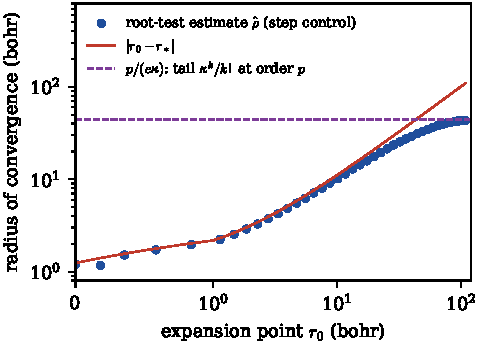
\includegraphics[width=\columnwidth]{fig_radius.pdf}
\caption{Radius of convergence of the local Taylor series of the helium orbital (run A of Table~\ref{tab:runs}). Points: the root-test estimate used for step control. Red line: the distance to the nearest singularities, located in Sec.~\ref{sec:analytic}. Dashed line: beyond about 20~bohr a finite order $p=\orderA$ sees the coefficients $\kappa^k/k!$ of the exponential tail first, which caps the estimate near $p/(e\kappa)=\plateau$~bohr.}
\label{fig:radius}
\end{figure}

Each step is a fixed fraction $c$ of the radius of convergence, estimated by the root test on the last nine coefficients, $\hat\rho=\min_{p-8\le k\le p}|f_0/f_k|^{1/k}$. The step $h=c\hat\rho$ is rounded down to a multiple of $2^{-16}$, so that every knot is an exact dyadic rational. Truncating the series then costs a relative error of about $c^p$, and we take $p=\lceil(d+5)/\log_{10}(1/c)\rceil$ for $d$ target digits. The radius grows linearly with distance from the nucleus (Fig.~\ref{fig:radius}), because it is the distance to a fixed pair of complex singularities. The steps therefore grow geometrically, and 51 steps reach $R=432$~bohr. We use $c=0.15$ by default; $c=0.25$ takes fewer steps at higher order.

\subsection{Shooting}

For fixed $a$, $f(R)$ depends almost linearly on $\mu$, because $\mu$ sets the amplitude of the solution growing as $e^{\kappa r}$. A secant iteration on $\mu$ (inner loop) therefore converges in two or three integrations. The normalisation residual $N(a)-1$, with the inner solve done for each $a$, is then smooth, and an outer secant iteration on $a$ solves it.

The natural alternative, a joint $2\times2$ Newton iteration on Eq.~\eqref{eq:conditions}, fails at large $R$. Away from the solution $N$ contains the growing mode squared, a term $\propto e^{2\kappa R}$, so its Jacobian row becomes parallel to that of $f(R)$. At $R=277$ in a 500-digit run the two rows were parallel to 31 digits, and the basin of the joint iteration shrinks as $e^{-\kappa R}$. The nested scalar solves never leave the growing mode in $N$, after the first few continuation stages, which take up to 60 integrations from the hydrogenic start, every stage takes 15--23, independent of $R$.

The wall is reached by continuation as we start from a screened hydrogenic orbital with $\zeta=Z-5/16$ and $R_0=7/\zeta$, and multiply $R$ by 1.2 per stage on a $1/64$ grid. Each stage targets the $d_k=\min(D,2\kappa R_k/\ln10)+10$ digits that its wall can deliver, with working precision $d_k+40$ digits, and updates $\kappa$ from the current $\varepsilon$. The mesh is frozen within a stage, so both residuals are smooth functions of $x$. The secant tolerance is $10^{-d_k}$, with initial relative offsets of $10^{-(d_k+40)/2}$.

%=====================================================================================
\section{Certification}\label{sec:certify}
%=====================================================================================

The shooting energy is accurate but not rigorous, being affected by rounding, series truncation and the secant tolerance. The certificate removes all three. It is a separate program of about 100 lines that shares no code with the solver, and it proceeds as follows.
\begin{enumerate}
\item It reads the elements $(r_j,h_j,\{f_{jk}\})$ written by the solver. All of these are dyadic rationals, since MPFR numbers are dyadic and the knots lie on a $2^{-16}$ grid. It verifies exactly that the elements tile $[0,R]$ ($r_0=0$, $h_j>0$, $r_j+h_j=r_{j+1}$).
\item On each element it substitutes $r=r_j+h_js$, $s\in[0,1]$, and multiplies by a common power of two so that every polynomial $P_j(s)$ has integer coefficients. The functional~\eqref{eq:functional} is invariant under this scaling.
\item It imposes continuity exactly, by setting $P_j(0)$ equal to $P_{j-1}(1)$, and the node $f(R)=0$, by adjusting the linear coefficient of the last element. Both adjustments are of the size of the solver's residuals, $\sim10^{-d}$. With $f=0$ beyond $R$, the trial function is a continuous piecewise polynomial with finite kinetic energy and therefore admissible.
\item It evaluates $N$, $T$, $V$ and $J$ of Eq.~\eqref{eq:integrals} exactly. On each element every integrand is an integer polynomial in $s$, integrated over $[0,1]$ with the common denominator $\mathrm{lcm}(1,\dots,n)$. The inner integral $Q(r)$ is accumulated across elements as an exact polynomial antiderivative.
\item It forms $E[f]$ as a rational number and prints it rounded towards $+\infty$.
\end{enumerate}
The variational principle then gives $\EHF\le E_R\le E[f]$ with no arithmetic error. Any piecewise polynomial would produce a valid bound; the solver only makes the bound tight. The cost is dominated by products of integer polynomials of degree $2p$ with coefficients of a few thousand bits: \certRunA~s at 120 digits and 34~min at 500. The current version computes these products by Kronecker substitution~\cite{vzGathen2013}: each polynomial is packed into one integer, so that GMP performs a single multiplication. It returns identical rationals 4--5 times faster at 100--200 digits; the helium timings quoted here predate it. Sec.~\ref{sec:be} extends the certificate to several orbitals.

%=====================================================================================
\section{Analytic structure of the orbital}\label{sec:analytic}
%=====================================================================================

\subsection{Complex singularities}

The hydrogenic orbital $e^{-Zr}$ is an entire function whilst the HF orbital is not: Eqs.~\eqref{eq:hf}--\eqref{eq:poisson} are nonlinear, and their solutions have movable singularities. Running B's Frobenius series at $r=0$, of order 626, shows sign patterns that rotate with $k$, which is the signature of a complex-conjugate pair. We fit the two-term recurrence $f_{k+1}=Af_k+Bf_{k-1}$ to its last 120 coefficients; the roots of $w^2-Aw-B$ are the reciprocals of the singular points. This gives
\begin{equation}
r_*=\rstar,\qquad |r_*|=\rstarabs\ \text{bohr}. \label{eq:rstar}
\end{equation}
The value changes by $\rstarerr$ between coefficient windows. Fits about $r_0=0.6$, 1.5, 3.5, 8 and 17~bohr locate the same pair to within $3\times10^{-2}$. Figure~\ref{fig:radius} confirms that the radius of convergence is $|r_0-r_*|$ along the whole inner region, which is what makes the Taylor steps grow geometrically.

\subsection{Consequences for single-exponent bases}

The $\Lambda$ functions of Refs.~\cite{Hatano2020,Hatano2025} are $L^{(2)}_n(2\zeta r)e^{-\zeta r}$, and our earlier basis~\cite{King2018} is of the same type. Expanding $f$ in them amounts to expanding $g(x)=f(x/2\zeta)\,e^{x/2}$ in Laguerre polynomials and the following two features of $f$ limit how fast the coefficients decay.
\begin{itemize}
\item \textbf{Tail mismatch.} The tail $e^{-\kappa r}$ becomes $e^{-\beta x}$ with $\beta=(\kappa-\zeta)/2\zeta$. The generating function $\sum_nL^{(\alpha)}_n(x)t^n=(1-t)^{-\alpha-1}e^{-xt/(1-t)}$ shows that its coefficients fall as $t^n$, with $|t|=(\zeta-\kappa)/(\zeta+\kappa)$.
\item \textbf{Singularity.} The singular point maps to $x_*=2\zeta r_*$. A Laguerre series converges inside the largest parabola $\mathrm{Re}\sqrt{-x}<\tau$ free of singularities, with coefficients decaying as $e^{-2\tau\sqrt n}$~\cite{Szego1975}. Here $\tau=\sqrt{2\zeta}\,\mathrm{Re}\sqrt{-r_*}=\tauHe\sqrt{2\zeta}$.
\end{itemize}
The energy error is quadratic in the orbital error, so the number of correct digits is about $(2/\ln10)\min\!\big[N\ln|t|^{-1},\,2\tau\sqrt N\big]$. Raising $\zeta$ pushes the singularity outward in $x$ but worsens the tail mismatch. The best exponent balances the two, giving $\zeta_\mathrm{opt}\propto N^{1/3}$ and an error $\exp(-cN^{2/3})$, slower than any geometric rate.

This leading-order estimate, which ignores prefactors, can be tested against the record calculation. For $N=150$ it gives $\zeta_\mathrm{opt}=\zetaopt$, against the numerically optimised $\zeta=5.1448$ of Ref.~\cite{Hatano2025}. At their exponent the two mechanisms limit the energy to \geoHatano\ and \singHatano\ digits respectively, so the optimised exponent indeed sits where they balance. The 66 digits observed are within the neglected prefactors. On the same estimate, 503 digits would need $N\approx\Nfive$ with $\zeta\approx\zetafive$, or about $10^{13}$ two-electron integrals at 500-digit precision which goes to show how efficient the FROST method is.

%=====================================================================================
\section{Results}\label{sec:results}
%=====================================================================================

\subsection{Helium}

\begin{table*}[t]
\caption{Helium runs. $D$: target digits; $R$: wall radius (bohr); $p$: Taylor order; $c$: step as a fraction of the radius of convergence; bits: MPFR working precision; steps: Taylor steps to $R$. Times are for one core of an Apple M4 Pro. The last two columns are $-\log_{10}|E-\EHF|/|\EHF|$ for the solver energy and for the certified bound, with run C as the reference.}
\label{tab:runs}
\begin{ruledtabular}
\begin{tabular}{lrrrrrrrrrr}
run & $D$ & $R$ & $p$ & $c$ & bits & steps & solver & certificate & solver s.f. & bound s.f. \\
\hline
A & 120 & 108.77 & 164 & 0.15 & 564 & 41 & 11~s & 16~s & 124.1 & 124.1 \\
B & 500 & 431.66 & 626 & 0.15 & 1827 & 51 & 7.4~min & 34~min & 503.2 & 503.2 \\
C & 500 & 445.00 & 856 & 0.25 & 1793 & 30 & 8.2~min & -- & reference & -- \\

\end{tabular}
\end{ruledtabular}
\end{table*}

\begin{figure}[t]
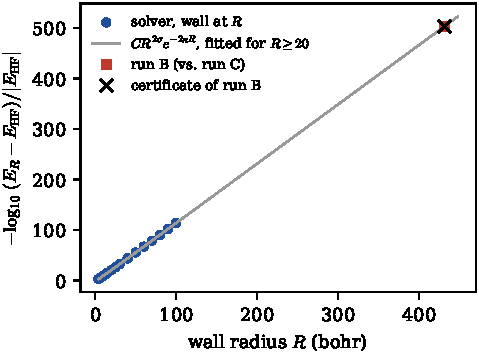
\includegraphics[width=\columnwidth]{fig_wall.pdf}
\caption{Accuracy of the confined energy $E_R$ against wall radius. Points up to $R=100$ are solver energies. The line is Eq.~\eqref{eq:wall} with $C$ fitted for $R\ge20$; it predicts run B's error at $R=432$ to 1\%. Square: run B against run C. Cross: the certified bound from run B.}
\label{fig:wall}
\end{figure}

Table~\ref{tab:runs} lists the helium runs. Run B (target 500 digits) and run C differ in wall radius, Taylor order, step fraction and working precision. The certificate of run B gives
\begin{equation}
\begin{split}
\EHF\le{}&\EHFsplit\ldots\ \eh ,
\end{split}\label{eq:bound}
\end{equation}
with the digits in full in Appendix~\ref{app:digits}. The error analysis follows.
\begin{itemize}
\item \textbf{The bound.} Eq.~\eqref{eq:bound} is rigorous. It lies $\certvsa$ from run B's own energy, so the adjustments of Sec.~\ref{sec:certify} are invisible at this precision.
\item \textbf{Its distance from $\EHF$.} Run B lies $\Eamb$ above run C. Eq.~\eqref{eq:wall}, fitted only to walls up to 100~bohr (Fig.~\ref{fig:wall}), predicts $\Eapred$ for run B's wall alone. The whole difference is therefore run B's wall. The same law gives $\Ecpred$ for run C's wall, and run C's truncation and rounding are set at 510 and 540 digits.
\item \textbf{Conclusion.} Hence $E[f]-\EHF=\gapcert$ to within about $10^{-509}$. That is a relative error of $10^{-\sfcert}$, and the first \Nsf\ significant figures of Eq.~\eqref{eq:bound} are those of $\EHF$.
\end{itemize}
As internal checks, run B satisfies the virial theorem to $|E+2T|=\virgap$. This is \virratio\ times its wall error, close to the ratio $2\kappa R=\twokR$ expected for the pressure term that a wall adds to the virial theorem. All 66 figures of Ref.~\cite{Hatano2025} agree with Eq.~\eqref{eq:bound}. The orbital energy is $\varepsilon=\epsHe\ldots$; Table~\ref{tab:series} gives more digits.

\subsection{The isoelectronic series}

\begin{table*}[t]
\caption{Closed-shell HF energies $\EHF$ and orbital energies $\varepsilon$ of the two-electron atoms (hartree), truncated. $R$ is the wall radius (bohr) of the certified 100-digit run. ``agree'' is $-\log_{10}$ of the relative difference between that run's exact certified bound and an independent solver run with a larger wall, $c=0.25$ and different working precision. Appendix~\ref{app:digits} gives the bounds rounded up to 100 significant figures.}
\label{tab:series}
\footnotesize
\begin{ruledtabular}
\begin{tabular}{rlllrr}
$Z$ & ion & $\EHF$ & $\varepsilon$ & $R$ & agree \\
\hline
1 & H$^-$ & \texttt{$-$0.48792\,97343\,70851\,74869\,28383\,72756\,80759\,06985} & \texttt{$-$0.04622\,24456\,27686\,93542\,6028} & 409.0 & 107.8 \\
2 & He & \texttt{$-$2.86167\,99956\,12238\,87877\,55437\,40022\,56342\,94128} & \texttt{$-$0.91795\,55628\,56339\,51014\,7216} & 91.8 & 104.2 \\
3 & Li$^+$ & \texttt{$-$7.23641\,52014\,52256\,24768\,29074\,24015\,50788\,80999} & \texttt{$-$2.79236\,44022\,45808\,08521\,9025} & 52.6 & 103.7 \\
4 & Be$^{2+}$ & \texttt{$-$13.61129\,94306\,19109\,03495\,58301\,80936\,76999\,6618} & \texttt{$-$5.66711\,55889\,28776\,00495\,431} & 36.9 & 103.5 \\
5 & B$^{3+}$ & \texttt{$-$21.98623\,44668\,24343\,01967\,70457\,83810\,15678\,7231} & \texttt{$-$9.54197\,84830\,02732\,90264\,850} & 28.5 & 103.3 \\
6 & C$^{4+}$ & \texttt{$-$32.36119\,28757\,18012\,33131\,52026\,75639\,74699\,5556} & \texttt{$-$14.41689\,16445\,67255\,25006\,614} & 23.2 & 103.3 \\
7 & N$^{5+}$ & \texttt{$-$44.73616\,39649\,42473\,12978\,20380\,85154\,85704\,6668} & \texttt{$-$20.29183\,17112\,25191\,51808\,053} & 19.5 & 103.3 \\
8 & O$^{6+}$ & \texttt{$-$59.11114\,27019\,13653\,85859\,84716\,50258\,65974\,1750} & \texttt{$-$27.16678\,78561\,29001\,32879\,335} & 16.9 & 103.2 \\
9 & F$^{7+}$ & \texttt{$-$75.48612\,64062\,60509\,83759\,56212\,09428\,90145\,1559} & \texttt{$-$35.04175\,43745\,26538\,66787\,855} & 14.9 & 103.2 \\
10 & Ne$^{8+}$ & \texttt{$-$93.86111\,35192\,31338\,15497\,81638\,81035\,30642\,9111} & \texttt{$-$43.91672\,79750\,63963\,31759\,665} & 13.3 & 103.2 \\

\end{tabular}
\end{ruledtabular}
\end{table*}

Only $Z$ changes along the series. Table~\ref{tab:series} lists certified 100-digit results for $Z=1$--10, each taking 10--16~s plus a certificate of similar cost. Every exact bound lies above its independent reference and agrees with it to 103--108 significant figures. Because $\kappa$ grows with $Z$, the wall needed for 100 digits shrinks from 409~bohr for H$^-$ to 13~bohr for Ne$^{8+}$.

\subsection{H$^-$}\label{sec:hminus}

H$^-$ is often described as unbound in HF theory. This means that $\EHF(\mathrm{H}^-)$ lies $\EAH\ \eh$ above the energy of H($1s$) plus a free electron, $-\tfrac12\ \eh$, so HF predicts a negative electron affinity. The closed-shell problem itself still has a normalisable solution. At large $r$ the Hartree potential $Y/r\to1/r$ cancels the nuclear attraction exactly, so the orbital sees a short-range potential deep enough to bind it: $\varepsilon=\epsH\ldots$ and $f\sim e^{-\kappa r}/r$ with $\kappa=\kappaH$ ($\sigma=0$ in Eq.~\eqref{eq:wall}).

The calculation shows this directly. The orbital energy converges to 15 digits by $R\approx76$~bohr and does not change as the wall moves out to 409~bohr, whereas an orbital held in place only by the wall would have $\varepsilon\to0$ as $R$ grows. The H$^-$ case lies just outside the existence theorem of Lieb and Simon, which needs fewer than $Z+1$ electrons~\cite{LiebSimon1977}. The certified value bounds the infimum of the closed-shell functional whether or not a minimiser exists. The closed-shell constraint is what keeps the ion together. Without it, a determinant with one electron in H($1s$) and the other spread out to infinity approaches $-\tfrac12\ \eh$, below the restricted energy. Because $\kappa$ is small, each significant figure costs 3.8~bohr of wall, against 0.85~bohr for helium.

\subsection{Correlation energy of helium}

Our FLAKE calculation~\cite{FLAKE} gives an upper bound on the nonrelativistic ground-state energy of helium, and estimates from convergence laws that the exact energy lies less than $3.3\times10^{-60}$ below it (60 significant figures). Subtracting $\EHF$ at either end of that interval gives the same correlation energy,
\begin{equation}
\begin{split}
E_\mathrm{corr}={}&\Ecorrsplit\ldots\ \eh,
\end{split}\label{eq:ecorr}
\end{equation}
correct to \Ncorr\ significant figures. Its accuracy is now set entirely by the correlated calculation.

\subsection{Computational cost}

All runs used Python with \texttt{gmpy2} (MPFR and GMP) on one core of an Apple M4 Pro.
\begin{itemize}
\item \textbf{Solver.} Each integration costs $O(p^2)$ multiplications per step at $d$-digit precision, with $p\propto d$ and $O(\log R)$ steps. There are $O(\log R)$ continuation stages of about 20 integrations each. The solver took 11~s at 120 digits and 7.4~min at 500, scaling as about $D^{2.6}$ over that range.
\item \textbf{Certificate.} It works with integers of up to a few thousand bits and scales as about $D^{3.4}$: 16~s at 120 digits and 34~min at 500.
\item \textbf{Memory.} The 500-digit orbital file, which holds every Taylor coefficient, is 18~MB so the memory footprint is very low.
\end{itemize}

%=====================================================================================
\section{Several $s$ orbitals: beryllium}\label{sec:be}
%=====================================================================================

\subsection{Equations}

For a closed shell of $n$ doubly occupied $s$ orbitals $f_i$, every pair of orbitals has a potential
\begin{equation}
Y_{ij}(r)=r\int_0^\infty\frac{f_i(s)f_j(s)\,s^2}{\max(r,s)}\,ds,\qquad Y_{ij}''=-rf_if_j,
\end{equation}
with $Y_{ij}(0)=0$ and $Y_{ij}'(R)=0$. $Y_{ii}$ is the Coulomb potential of orbital $i$ and $Y_{ij}$ ($i\ne j$) the exchange potential between $i$ and $j$. For $s$ orbitals only the monopole term appears, so in this form exchange is a multiplication, not an integral operator. The canonical HF equations generalise Eq.~\eqref{eq:hf} to
\begin{equation}
rf_i''+2f_i'=2\Big[\Big(\sum_j2Y_{jj}-Y_{ii}-Z-\varepsilon_ir\Big)f_i-\sum_{j\ne i}Y_{ij}f_j\Big]. \label{eq:ns}
\end{equation}
As for helium, $Y_{ij}=b_{ij}r+\tilde Y_{ij}$, so the orbitals depend on $\varepsilon_i$ and $b_{ij}$ only through $\mu_i=\varepsilon_i-\sum_j2b_{jj}+b_{ii}$ and $\nu_{ij}=b_{ij}$ ($i\ne j$). The Taylor recurrences of Sec.~\ref{sec:numerics} carry over term by term, and the Frobenius series again gives $f_i'(0)=-Zf_i(0)$. Beryllium ($n=2$) has two orbitals, three pair potentials and five shooting parameters, $(a_1,a_2,\mu_1,\mu_2,\nu_{12})$ with $a_i=f_i(0)$. With $n=1$ the same code reproduces the helium results.

\subsection{One wall per orbital}

The $1s$ orbital decays as $e^{-\kappa_1r}$ with $\kappa_1=\BeKappaOne$, the $2s$ as $e^{-\kappa_2r}$ with $\kappa_2=\BeKappaTwo$. A single wall placed for the $2s$ would make the $1s$ growing mode $e^{\kappa_1r}$ demand $\kappa_1/\kappa_2\approx4$ times the working precision. Each orbital therefore has its own wall $R_i$, chosen so that $e^{-2\kappa_iR_i}$ is the same for all, and is zero beyond it; for the run of Eq.~\eqref{eq:bebound} below, $R_1=\BeRone$ and $R_2=\BeRtwo$~bohr. These orbitals are still admissible, so the variational bound is unaffected.

\subsection{Canonical orbitals and a certificate without orthogonality}

With a common wall, canonical orbitals of one Fock operator are orthogonal automatically. With unequal walls they are not, and the constrained optimum needs a Lagrange multiplier, a term $\lambda_{12}rf_j$ in each equation. Enforcing exact orthogonality with it proved badly conditioned. The overlap $S_{12}$ responds to $\lambda_{12}$ only at the $10^{-4}$ level, and a Newton step large enough to correct it forces a $1s$ tail far above its natural size $e^{-\kappa_1R_1}$, which the exchange term passes into the $2s$ growing mode. We keep the canonical equations instead ($\lambda_{12}=0$, so $\nu_{12}=b_{12}$ is fixed by $Y_{12}'(R)=0$) and accept the overlap that results: $|S_{12}|=\BeSij$ for the run of Eq.~\eqref{eq:bebound}. Because the energy is stationary, the cost is of order $S_{12}^2$, far below the wall error.

The certificate makes this rigorous. For any orbitals, orthonormal or not, the closed-shell determinant energy is
\begin{equation}
\begin{split}
E={}&2\sum_{ij}P_{ij}h_{ij}\\
&+\sum_{ijkl}P_{ij}P_{kl}\big[2(ij|kl)-(ik|jl)\big],
\end{split}\label{eq:nonorth}
\end{equation}
with $P=S^{-1}$. It depends only on the span of the orbitals. For piecewise polynomials every overlap $S_{ij}$, one-electron integral $h_{ij}$ and two-electron integral $(ij|kl)=\int\rho_{ij}rQ_{kl}\,dr+\int\rho_{kl}rQ_{ij}\,dr$ (with $\rho_{ij}=f_if_j$ and $Q_{kl}(r)=\int_0^r\rho_{kl}s^2ds$) is a rational number, computed as in Sec.~\ref{sec:certify}, and $S^{-1}$ is inverted exactly. For $n=1$, Eq.~\eqref{eq:nonorth} reduces to Eq.~\eqref{eq:functional}, and the generalised certifier returns the identical rational for helium.

\subsection{Shooting}

Two further changes were needed.
\begin{itemize}
\item \textbf{Nested solves from the innermost orbital outward.} Solving $f_1(R_1)=0$ and $f_2(R_2)=0$ jointly fails. While $\mu_1$ is wrong, the $1s$ orbital carries a growing mode that the exchange term feeds into the $2s$ equation, and $f_2(R_2)$ acquires spurious roots in $\mu_2$. Every trial $\mu_2$ therefore re-solves $\mu_1$ first. The $1s$ rounding error that remains is amplified near $R_1$ and passed on through exchange, which limits $\mu_2$ to about $10^{-0.6d}$. The energy, quadratic in orbital errors, is unaffected, so the scalar solves stop when the residual reaches its noise floor. The outer unknowns $(a_1,a_2,\nu_{12})$ are found by Broyden's method from a fresh finite-difference Jacobian at each wall radius; a Jacobian carried over from the previous radius converges only linearly.
\item \textbf{Homotopy start.} Screened hydrogenic orbitals are too crude a start for the $2s$. We scale the electron--electron terms by $t$ and follow the solution from $t=0$, where the orbitals are hydrogenic and exact, to $t=1$ in 40 steps at low precision with a linear predictor.
\end{itemize}

\subsection{Results}

\begin{table*}[t]
\caption{Beryllium runs. Run A$_D$ targets $D$ digits and is certified; run B$_D$ is an independent check with larger walls, $c=0.25$ and hence a different Taylor order and mesh. $R_1$, $R_2$: walls of the $1s$ and $2s$ orbitals (bohr); other columns as in Table~\ref{tab:runs}, with run B\BeRef\ as the reference. Runs were made up to four at a time on the same laptop.}
\label{tab:beruns}
\begin{ruledtabular}
\begin{tabular}{lrrrrrrrrrrr}
run & $D$ & $R_1$ & $R_2$ & $p$ & $c$ & bits & steps & solver & certificate & solver s.f. & bound s.f. \\
\hline
A100 & 100 & 40.4 & 158.1 & 140 & 0.15 & 498 & 54 & 175~s & 18~s & 103.0 & 103.0 \\
B100 & 110 & 44.2 & 172.8 & 208 & 0.25 & 498 & 32 & 299~s & -- & 112.9 & -- \\
A200 & 200 & 77.8 & 304.5 & 261 & 0.15 & 830 & 59 & 23~min & 86~s & 202.3 & 202.3 \\
B200 & 210 & 81.6 & 319.1 & 374 & 0.25 & 830 & 34 & 21~min & -- & 212.2 & -- \\
A500 & 500 & 190.1 & 743.7 & 626 & 0.15 & 1827 & 65 & 240~min & 13~min & 501.3 & 501.3 \\
B500 & 510 & 193.9 & 758.3 & 873 & 0.25 & 1827 & 38 & 233~min & -- & reference & -- \\

\end{tabular}
\end{ruledtabular}
\end{table*}

\begin{table*}[t]
\caption{Published Hartree--Fock energies of the beryllium ground state (hartree), as compiled in Table~4 of Ref.~\cite{Hatano2025} and truncated there to their significant figures; our row shows the first 66 of \BeNsf\ correct figures.}
\label{tab:behist}
\footnotesize
\begin{ruledtabular}
\begin{tabular}{rlll}
year & authors & energy & s.f. \\
\hline
1995 & Koga \textit{et al.}~\cite{Koga1995} & \texttt{$-$14.57302\,317} & 10 \\
2001 & Andrae, Brodbeck, Hinze~\cite{Andrae2001} & \texttt{$-$14.57302\,317} & 10 \\
2009 & Saito~\cite{Saito2009} & \texttt{$-$14.57302\,31683} & 12 \\
2019 & Lehtola~\cite{Lehtola2019} & \texttt{$-$14.57302\,3168} & 11 \\
2020 & Cinal~\cite{Cinal2020} & \texttt{$-$14.57302\,31683\,16399\,58241\,145} & 25 \\
2022 & Hatano, Yamamoto~\cite{Hatano2022} & \texttt{$-$14.57302\,31683\,16399\,58241\,14473\,599} & 30 \\
2025 & Hatano, Yamamoto~\cite{Hatano2025} & \texttt{$-$14.57302\,31683\,16399\,58241\,14473\,59870\,01445\,38777\,2} & 43 \\
2026 & This work & \texttt{$-$14.57302\,31683\,16399\,58241\,14473\,59870\,01445\,38777\,21357\,77400\,54138\,05222\,7220\dots} & 501 \\

\end{tabular}
\end{ruledtabular}
\end{table*}

Table~\ref{tab:beruns} lists the runs. The certificate of run A\BeRef\ gives
\begin{equation}
\begin{split}
\EHF(\mathrm{Be})\le{}&\BeEsplit\ldots\ \eh ,
\end{split}\label{eq:bebound}
\end{equation}
with all digits in Appendix~\ref{app:digits}. It lies $\BeGap$ above run B\BeRef. Eq.~\eqref{eq:wall} for the $2s$ wall, with $\sigma=1/\kappa_2$ in the residual field $-1/r$ and $C$ fitted to run A\BeWallFrom\ alone, predicts $\BeWallPred$ for run A\BeRef's wall. The difference is therefore the wall error of the certified run, and its relative size, $10^{-\BeSfcert}$, makes the first \BeNsf\ significant figures of Eq.~\eqref{eq:bebound} those of $\EHF(\mathrm{Be})$. All 43 figures of Ref.~\cite{Hatano2025} agree (Table~\ref{tab:behist}). The orbital energies are $\varepsilon_{1s}=\BeEpsOne\ldots$ and $\varepsilon_{2s}=\BeEpsTwo\ldots$. The run took \BeTime\ and its certificate \BeCertTime.

%=====================================================================================
\section{Quality of the orbitals}\label{sec:orbitals}
%=====================================================================================

The energy is often a forgiving test for method accuracy as it is stationary, so an orbital error of relative size $\delta$ changes it only at order $\delta^2$, whereas every other property changes at order $\delta$. In a basis-set calculation, properties therefore carry far fewer correct figures than the energy, and fewest near the nucleus. At the 66-figure energy of Ref.~\cite{Hatano2025}, the cusp ratio of helium has 30 correct figures, $\rho(0)$ 32 and $\langle r^{-2}\rangle$ 35 (Table~\ref{tab:props}). FROST orbitals behave differently, because their only error is the wall and that error is known in closed form. We evaluate properties of the same exact trial orbitals that are certified, by exact integration of the piecewise polynomials.

\begin{table*}[t]
\caption{Orbital properties per electron, compared with the multiple-precision $\Lambda$-function results of Ref.~\cite{Hatano2025} (its Tables 4 and 6). CC is the cusp ratio $\rho'(0)/2\rho(0)$ (exactly $-Z$), VR the virial ratio $V/T$ (exactly $-2$), $\rho(0)$ the total density at the nucleus, and $\langle r^k\rangle$ is in bohr$^k$. Values are truncated to 22 figures. ``here'' is the number of correct significant figures, from the relative difference between our two independent runs (He: runs B and C; Be: runs A\BeRef\ and B\BeRef), and for VR from the virial ratio of run B (He) or A\BeRef\ (Be). ``Ref.'' is the number reported in Ref.~\cite{Hatano2025}; every figure printed there agrees with ours, up to rounding of the last.}
\label{tab:props}
\footnotesize
\begin{ruledtabular}
\begin{tabular}{llrrlrr}
& \multicolumn{3}{c}{He} & \multicolumn{3}{c}{Be} \\
property & value & here & Ref. & value & here & Ref. \\
\hline
CC & $-2$ (exact) & exact & 30 & $-4$ (exact) & exact & 19 \\
VR & $-2$ & 500 & 68 & $-2$ & 498 & 55 \\
$\rho(0)$ & \texttt{3.59591\,82637\,62248\,92070\,6}\dots & 500 & 32 & \texttt{35.38771\,67410\,93786\,44935}\dots & 498 & 20 \\
$\langle r^{-2}\rangle$ & \texttt{5.99550\,36673\,12524\,59727\,3}\dots & 500 & 35 & \texttt{14.40450\,64454\,41573\,89932}\dots & 498 & 23 \\
$\langle r^{-1}\rangle$ & \texttt{1.68728\,22152\,81009\,40400\,8}\dots & 500 & 65 & \texttt{2.10219\,94129\,30678\,79400\,7}\dots & 498 & 41 \\
$\langle r\rangle$ & \texttt{0.92727\,34047\,31493\,19741\,89}\dots & 497 & 63 & \texttt{1.53220\,39722\,81112\,53930\,2}\dots & 495 & 39 \\
$\langle r^{2}\rangle$ & \texttt{1.18482\,84799\,09482\,92632\,5}\dots & 495 & 61 & \texttt{4.32969\,28432\,10096\,87398\,1}\dots & 492 & 38 \\
$\langle r^{3}\rangle$ & \texttt{1.94063\,62073\,75593\,29252\,7}\dots & 493 & 60 & \texttt{15.78772\,44502\,52942\,44512}\dots & 490 & 37 \\
$\langle r^{4}\rangle$ & \texttt{3.88794\,66255\,72633\,62739\,1}\dots & 491 & 58 & \texttt{67.66413\,23859\,49548\,84927}\dots & 488 & 35 \\
$\langle r^{5}\rangle$ & \texttt{9.22119\,73006\,38698\,13804\,8}\dots & 488 & 57 & \texttt{331.37292\,59118\,13439\,5126}\dots & 486 & 34 \\
$\langle r^{6}\rangle$ & \texttt{25.27839\,04132\,93347\,64158}\dots & 486 & 56 & \texttt{1826.40384\,40394\,25393\,288}\dots & 484 & 33 \\
$\langle r^{7}\rangle$ & \texttt{78.65249\,19190\,10120\,85779}\dots & 484 & 54 & \texttt{11199.59304\,93608\,21497\,21}\dots & 482 & 32 \\
$\langle r^{8}\rangle$ & \texttt{273.84506\,80901\,48372\,3311}\dots & 482 & 53 & \texttt{75677.78895\,46800\,29670\,81}\dots & 480 & 31 \\
$\langle r^{9}\rangle$ & \texttt{1054.83264\,42597\,84461\,806}\dots & 480 & 52 & \texttt{558916.88019\,33108\,60490\,3}\dots & 478 & 30 \\

\end{tabular}
\end{ruledtabular}
\end{table*}

\subsection{The nucleus}

The first step of the Frobenius recurrence is $f_1=-Zf_0$ (Sec.~\ref{sec:numerics}). For $Z=2$ and $Z=4$ it involves no rounding, so the cusp ratio $f'(0)/f(0)$ of every certified orbital, both beryllium orbitals included, is exactly the rational number $-Z$, and so is $\rho'(0)/2\rho(0)$. The higher Frobenius coefficients also come from the HF equation itself, so the orbital has the analytic form of the HF solution at the nucleus, not merely the right cusp. The properties dominated by this region are then as accurate as any other. Runs B and C give the same $\rho(0)$ to \PropRho\ significant figures and the same $\langle r^{-2}\rangle$ to \PropRtwo.

\subsection{Pointwise error}

Once the density has decayed, $Y=1$ up to terms of order $e^{-2\kappa r}$, and Eq.~\eqref{eq:hf} becomes the Coulomb equation for charge $Z-1$ at energy $\varepsilon$. Its decaying and growing solutions are $W_{\sigma,1/2}(2\kappa r)/r$ and $M_{\sigma,1/2}(2\kappa r)/r$, where $W$ and $M$ are Whittaker functions~\cite{DLMF}. The free orbital is $A\,W_{\sigma,1/2}(2\kappa r)/r$. A wall at $R$ adds the multiple of the growing solution that makes $f$ vanish there, so the relative error of the confined orbital is
\begin{equation}
\frac{f_R}{f}-1\simeq-\frac{W_{\sigma,\frac12}(2\kappa R)\,M_{\sigma,\frac12}(2\kappa r)}{M_{\sigma,\frac12}(2\kappa R)\,W_{\sigma,\frac12}(2\kappa r)}\propto\Big(\frac Rr\Big)^{2\sigma}e^{-2\kappa(R-r)}, \label{eq:pointwise}
\end{equation}
plus a constant of the order of the energy error from the shifts of $\varepsilon$ and of the normalisation. Figure~\ref{fig:local} compares Eq.~\eqref{eq:pointwise} for run B with the measured difference between runs B and C. From $r=10$~bohr out to the wall they agree to one part in $10^{\PredParts}$. Run B's orbital is therefore correct to 500 figures at the nucleus and to about 250 at $r=R/2$, and its error is known everywhere.

\begin{figure}[t]
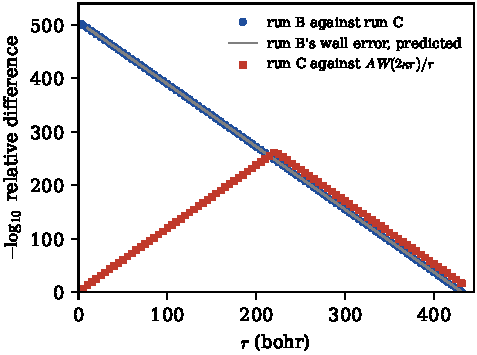
\includegraphics[width=\columnwidth]{fig_local.pdf}
\caption{Pointwise accuracy of the 500-digit helium orbital. Circles: relative difference between runs B ($R=431.7$) and C ($R=445$). Line: run B's wall error predicted by Eq.~\eqref{eq:pointwise}. Squares: run C against the exact Coulomb tail $A\,W_{\sigma,1/2}(2\kappa r)/r$, limited at small $r$ by the non-Coulomb part of the potential and at large $r$ by the wall.}
\label{fig:local}
\end{figure}

The same figure tests the tail itself. Run C, divided by $A\,W_{\sigma,1/2}(2\kappa r)/r$ with $A$ fitted at $r=\Rfit$~bohr, approaches 1 as $e^{-2\kappa r}$ while the exponentially small part of the Hartree potential dies away. Near $r=R/2$, where this error meets the growing wall error, the agreement reaches about \TailBest\ significant figures. The decay constant, the power $r^{\sigma-1}$ and every correction to it are thus those of the exact Coulomb tail. The asymptotic normalisation of the helium HF orbital, with $\int f^2r^2\,dr=1$, is $A=\Aasym\ldots$

\subsection{Expectation values}

Because $M_{\sigma,1/2}W_{\sigma,1/2}$ tends to a constant, Eq.~\eqref{eq:pointwise} changes $f^2r^2$ by the same amount $u$ at every $r$ in the Coulomb region. Then $\delta\langle r^k\rangle\approx u\,[R^{k+1}/(k+1)-R\langle r^k\rangle]$, and each power of $r$ costs about $\log_{10}R-\log_{10}(\langle r^{k+1}\rangle/\langle r^k\rangle)\approx2$ significant figures. With $u$ fitted at $k=1$, this reproduces the differences between runs B and C for every $k$ from 1 to 12 to within \UniPct\%, and even $\langle r^{12}\rangle$ is correct to \PropRtwelve\ figures. Table~\ref{tab:props} lists the results beside those of Ref.~\cite{Hatano2025}. The virial ratio of run B deviates from $-2$ only by its wall pressure (Sec.~\ref{sec:results}), at the $10^{-\PropVR}$ level. For beryllium we take $T$ from each orbital normalised on its own; the kinetic energy of the $P=S^{-1}$ determinant, like any property, is good only to about $|S_{12}|$.

\subsection{Beryllium}

Both beryllium cusp ratios are exactly $-4$, against 19 correct figures in Ref.~\cite{Hatano2025}. Runs A\BeRef\ and B\BeRef\ agree on $\rho(0)$ to \BeRho\ figures and on the $\langle r^k\rangle$ of the density to \BeDensMin--\BeDensMax, the wall error of run A\BeRef. The moments of the individual $1s$ and $2s$ orbitals agree only to \BeOrbMin--\BeOrbMax\ figures, comparable to $|S_{12}|=\BeSij$. This is consistent with a rotation of order $S_{12}$ within the occupied space, which leaves the determinant and its density unchanged to first order. Physical properties depend only on the density, and the per-electron averages of Table~\ref{tab:props} are density properties.

%=====================================================================================
\section{Discussion}
%=====================================================================================

For closed-shell atoms whose occupied orbitals are all $s$ orbitals, the HF problem is one-dimensional, and it can be solved to essentially any precision in time polynomial in the number of digits. This needs no basis set, no two-electron integrals and no extrapolation. The only approximation is the wall, whose error decays exponentially and follows a law (Eq.~\eqref{eq:wall}) that is verified independently. The solver and the certificate play separate roles. The solver is free to use any arithmetic or heuristic, because the certificate turns its output into a bound that depends on nothing but exact integer arithmetic and the variational principle. The same construction applies whenever an energy functional is an integral of polynomials in the trial function: a piecewise polynomial with dyadic coefficients always admits an exact evaluation.

Beryllium shows that the method is not specific to two electrons. Each pair of occupied orbitals adds a Poisson equation and each orbital adds a shooting parameter. The problems this creates, an inner orbital's growing mode and the coupling through exchange, were solved by giving each orbital its own wall, by solving from the innermost orbital outward, and by a certificate that does not need orthogonality. For $p$ and $d$ shells, exchange brings multipoles $r_<^k/r_>^{k+1}$ with $k\ge1$. Their integrals over a polynomial element produce logarithms of knot ratios, so the certificate would need rigorous interval enclosures of those logarithms instead of exact rationals; the solver is unchanged. Open shells such as lithium need the restricted open-shell energy expression. The Be-like ions follow from Sec.~\ref{sec:be} by changing $Z$.

The main limitation is that the bound is one-sided. The distance to $\EHF$ is established by an independent run and by the measured wall law, not by a rigorous lower bound. Producing a certified lower bound for a nonlinear eigenproblem at this precision remains open.

\section*{Data and code availability}
The solvers (\texttt{oracle.py} for one orbital, \texttt{oracle\_ns.py} for several), the certificate (\texttt{certify.py}), orbital properties (\texttt{properties.py}), a test, the 100-digit isoelectronic values and the script generating every table and figure of this paper are in Ref.~\cite{code}.

% \begin{acknowledgments}
% TODO: acknowledgments (and any disclosure of AI assistance required by the venue).
% \end{acknowledgments}

\appendix
\section{Digits}\label{app:digits}

\begin{widetext}
The certified bound for helium from run B, truncated to its \Nsf\ correct significant figures (truncation keeps every value here an upper bound):
\[\begin{aligned}E_\mathrm{HF}(\mathrm{He})\le{}&-2.
8616799956\,1223887877\,5543740022\,5634294128\,7977675244\\ &\hphantom{-2.}7053906864\,6974341883\,6262795569\,6043994965\,3409977869\\ &\hphantom{-2.}0984175165\,7319012702\,3919647238\,6125667693\,7899153381\\ &\hphantom{-2.}1865805702\,9646754000\,6262349883\,4061443950\,9601437492\\ &\hphantom{-2.}4135358476\,7851824834\,0821214097\,0971618545\,3258894677\\ &\hphantom{-2.}1779765923\,3024533037\,8073662227\,1074836399\,7217257536\\ &\hphantom{-2.}6709739632\,5040135317\,3639891864\,9058074245\,0858489821\\ &\hphantom{-2.}0511928945\,7211993802\,4044762317\,9624760205\,8266331292\\ &\hphantom{-2.}1264856378\,6408084536\,2955571466\,4474164321\,9393621412\\ &\hphantom{-2.}5615947217\,4331793223\,0647798571\,8919570787\,0010781657\\ &\hphantom{-2.}47\ldots\end{aligned}\]

The certified bound for beryllium from run A500, truncated to its 501 correct significant figures:
\[\begin{aligned}E_\mathrm{HF}(\mathrm{Be})\le{}&-14.
5730231683\,1639958241\,1447359870\,0144538777\,2135777400\\ &\hphantom{-14.}5413805222\,7220687300\,0193822635\,1455080316\,9376936498\\ &\hphantom{-14.}9813411646\,0590414220\,8100746275\,1047907294\,5277805073\\ &\hphantom{-14.}8975228184\,9318054044\,5506276329\,3865670096\,0809617754\\ &\hphantom{-14.}8999876512\,9672202879\,1450889866\,6849101213\,4508707507\\ &\hphantom{-14.}9427000347\,0399581021\,8875529001\,2123902027\,0945596918\\ &\hphantom{-14.}4619912969\,1544989534\,9196332042\,5651173890\,8727366296\\ &\hphantom{-14.}9171855704\,7823504902\,4927158415\,9882076703\,9342895408\\ &\hphantom{-14.}1793383926\,2557682238\,9455941180\,4164488745\,9691458140\\ &\hphantom{-14.}6525412122\,2562597650\,3205668895\,2590379295\,553928939\ldots\end{aligned}\]

The certified bounds for the two-electron isoelectronic series, rounded up to 100 significant figures:

\begin{tabular}{rll}
$Z$ & ion & $E_\mathrm{HF}$ (hartree) \\ \hline
1 & H$^-$ & \texttt{$-$0.4879297343 7085174869 2838372756 8075906985 3910785709} \\
 & & \texttt{\phantom{$-$0.}6269038281 1340665609 7897185876 8966814715 5846566757} \\
2 & He & \texttt{$-$2.8616799956 1223887877 5543740022 5634294128 7977675244} \\
 & & \texttt{\phantom{$-$2.}7053906864 6974341883 6262795569 6043994965 340997786} \\
3 & Li$^+$ & \texttt{$-$7.2364152014 5225624768 2907424015 5078880999 6155485795} \\
 & & \texttt{\phantom{$-$7.}0494422097 9096948083 9824349926 8208719101 959449017} \\
4 & Be$^{2+}$ & \texttt{$-$13.6112994306 1910903495 5830180936 7699966184 6449778750} \\
 & & \texttt{\phantom{$-$13.}8490544069 2629053406 9058737132 8045073910 84123264} \\
5 & B$^{3+}$ & \texttt{$-$21.9862344668 2434301967 7045783810 1567872310 6164671870} \\
 & & \texttt{\phantom{$-$21.}4966978607 1405795390 7507459393 2780368884 77734442} \\
6 & C$^{4+}$ & \texttt{$-$32.3611928757 1801233131 5202675639 7469955566 8383224096} \\
 & & \texttt{\phantom{$-$32.}7460246834 1345694182 6975127407 2131126585 40991441} \\
7 & N$^{5+}$ & \texttt{$-$44.7361639649 4247312978 2038085154 8570466688 6590871341} \\
 & & \texttt{\phantom{$-$44.}6298429652 2643541074 4982503068 5743194168 15832539} \\
8 & O$^{6+}$ & \texttt{$-$59.1111427019 1365385859 8471650258 6597417502 6580481271} \\
 & & \texttt{\phantom{$-$59.}9121555099 4989409315 4057585162 9328732427 93226341} \\
9 & F$^{7+}$ & \texttt{$-$75.4861264062 6050983759 5621209428 9014515596 0041484019} \\
 & & \texttt{\phantom{$-$75.}1470841147 8116942143 1274221352 6242319785 50956336} \\
10 & Ne$^{8+}$ & \texttt{$-$93.8611135192 3133815497 8163881035 3064291112 8543638382} \\
 & & \texttt{\phantom{$-$93.}1944783379 8796142782 0812917287 1166295321 85129503} \\
\end{tabular}

\end{widetext}

\begin{thebibliography}{99}
\bibitem{Hartree1928} D. R. Hartree, Proc. Camb. Phil. Soc. \textbf{24}, 89 (1928).
\bibitem{Slater1928} J. C. Slater, Phys. Rev. \textbf{32}, 339 (1928).
\bibitem{Fock1930} V. Fock, Z. Phys. \textbf{61}, 126 (1930).
\bibitem{Slater1930} J. C. Slater, Phys. Rev. \textbf{35}, 210 (1930).
\bibitem{Slater1929} J. C. Slater, Phys. Rev. \textbf{34}, 1293 (1929).
\bibitem{Hartree1935} D. R. Hartree and W. Hartree, Proc. R. Soc. Lond. A \textbf{150}, 9 (1935).
\bibitem{Hartree1957} D. R. Hartree, \textit{The Calculation of Atomic Structures} (Wiley, New York, 1957).
\bibitem{Roothaan1951} C. C. J. Roothaan, Rev. Mod. Phys. \textbf{23}, 69 (1951).
\bibitem{Hall1951} G. G. Hall, Proc. R. Soc. Lond. A \textbf{205}, 541 (1951).
\bibitem{Boys1950} S. F. Boys, Proc. R. Soc. Lond. A \textbf{200}, 542 (1950).
\bibitem{Moller1934} C. M{\o}ller and M. S. Plesset, Phys. Rev. \textbf{46}, 618 (1934).
\bibitem{Cizek1966} J. \v{C}\'{\i}\v{z}ek, J. Chem. Phys. \textbf{45}, 4256 (1966).
\bibitem{KohnSham1965} W. Kohn and L. J. Sham, Phys. Rev. \textbf{140}, A1133 (1965).
\bibitem{Becke1993} A. D. Becke, J. Chem. Phys. \textbf{98}, 5648 (1993).
\bibitem{Lowdin1959} P.-O. L\"owdin, Adv. Chem. Phys. \textbf{2}, 207 (1959).
\bibitem{FroeseFischer1977} C. Froese Fischer, \textit{The Hartree--Fock Method for Atoms: A Numerical Approach} (Wiley, New York, 1977).
\bibitem{Roothaan1960} C. C. J. Roothaan, L. M. Sachs, and A. W. Weiss, Rev. Mod. Phys. \textbf{32}, 186 (1960).
\bibitem{Clementi1974} E. Clementi and C. Roetti, At. Data Nucl. Data Tables \textbf{14}, 177 (1974).
\bibitem{Gazquez1977} J. L. G\'azquez and H. J. Silverstone, J. Chem. Phys. \textbf{67}, 1887 (1977).
\bibitem{Szalewicz1981} K. Szalewicz and H. J. Monkhorst, J. Chem. Phys. \textbf{75}, 5785 (1981).
\bibitem{Koga1995} T. Koga, S. Watanabe, K. Kanayama, R. Yasuda, and A. J. Thakkar, J. Chem. Phys. \textbf{103}, 3000 (1995).
\bibitem{Andrae2001} D. Andrae, R. Brodbeck, and J. Hinze, Int. J. Quantum Chem. \textbf{82}, 227 (2001).
\bibitem{Saito2009} S. L. Saito, At. Data Nucl. Data Tables \textbf{95}, 836 (2009).
\bibitem{King2018} A. W. King, A. L. Baskerville, and H. Cox, Phil. Trans. R. Soc. A \textbf{376}, 20170153 (2018).
\bibitem{Lehtola2019} S. Lehtola, Int. J. Quantum Chem. \textbf{119}, e25945 (2019).
\bibitem{Cinal2020} M. Cinal, J. Math. Chem. \textbf{58}, 1571 (2020).
\bibitem{Hatano2020} Y. Hatano and S. Yamamoto, J. Phys. Commun. \textbf{4}, 085006 (2020).
\bibitem{Hatano2022} Y. Hatano and S. Yamamoto, Mol. Phys. \textbf{120}, e2027534 (2022).
\bibitem{Hatano2025} Y. Hatano and S. Yamamoto, J. Comput. Chem. Jpn. Int. Ed. \textbf{11}, 2024-0032 (2025).
\bibitem{vzGathen2013} J. von zur Gathen and J. Gerhard, \textit{Modern Computer Algebra}, 3rd ed. (Cambridge University Press, Cambridge, 2013).
\bibitem{MPFR} L. Fousse, G. Hanrot, V. Lef\`evre, P. P\'elissier, and P. Zimmermann, ACM Trans. Math. Softw. \textbf{33}, 13 (2007).
\bibitem{Corliss1982} G. Corliss and Y. F. Chang, ACM Trans. Math. Softw. \textbf{8}, 114 (1982).
\bibitem{Jorba2005} \`A. Jorba and M. Zou, Exp. Math. \textbf{14}, 99 (2005).
\bibitem{Moore1966} R. E. Moore, \textit{Interval Analysis} (Prentice-Hall, Englewood Cliffs, NJ, 1966).
\bibitem{Kato1957} T. Kato, Commun. Pure Appl. Math. \textbf{10}, 151 (1957).
\bibitem{Janes2011} P. P. Janes and A. P. Rendell, J. Chem. Theory Comput. \textbf{7}, 1631 (2011).
\bibitem{code} A. L. Baskerville, \texttt{frost}: \url{https://github.com/adambaskerville/frost}.
\bibitem{LiebSimon1977} E. H. Lieb and B. Simon, Commun. Math. Phys. \textbf{53}, 185 (1977).
\bibitem{Szego1975} G. Szeg\H{o}, \textit{Orthogonal Polynomials}, 4th ed. (American Mathematical Society, Providence, RI, 1975).
\bibitem{FLAKE} A. L. Baskerville, ChemRxiv (2026), doi:10.26434/chemrxiv.15010182.
\bibitem{DLMF} F. W. J. Olver \textit{et al.}, eds., \textit{NIST Digital Library of Mathematical Functions}, Chap.~13, \url{https://dlmf.nist.gov/13}.
\end{thebibliography}

\end{document}
